\documentclass[main.tex]{subfiles}

\begin{document}
\section{The PCT Project}
\textit{This chapter covers the PCT-project that is currently under development at the Department of physics and technology in Bergen. It discusses the DTC being developed for the project, and how it tracks and measures the energy protons. Finally, a technical overview of the system is given, along with how the Power Control System and the control software of this thesis will be implemented.}

The Bergen \gls{pct}-project is a collaboration between the University of Bergen and several other institutions worldwide. The purpose is to build a \gls{pct}-scanner to be used in measuring \gls{rsp}. The design is based on using a \acrlong{dtc} to detect protons emitted from a particle accelerator. In particular, the focus is on creating a scanner for use on pediatric patients.


\subsection{Introduction}

The \gls{pct}-project comprises several control systems and sensors. The main instrument is a \gls{dtc} that uses \gls{alpide}-chips to measure the energy of protons. The \gls{dtc} is made out of 43 layers of \gls{alpide} sensors and there are three control systems that oversee the \gls{dtc}. These systems are cooling, readout, and power delivery. The cooling system is connected directly to the \gls{dtc}, while power delivery and readout perform their actions through a \gls{tc}. All systems are connected to a network that allows them to communicate with the Control Room.

The \gls{pct}-system is still under development, \autoref{fig: pct_diagram} shows the current implementation of the system.

\begin{figure}[!ht]
    \centering
    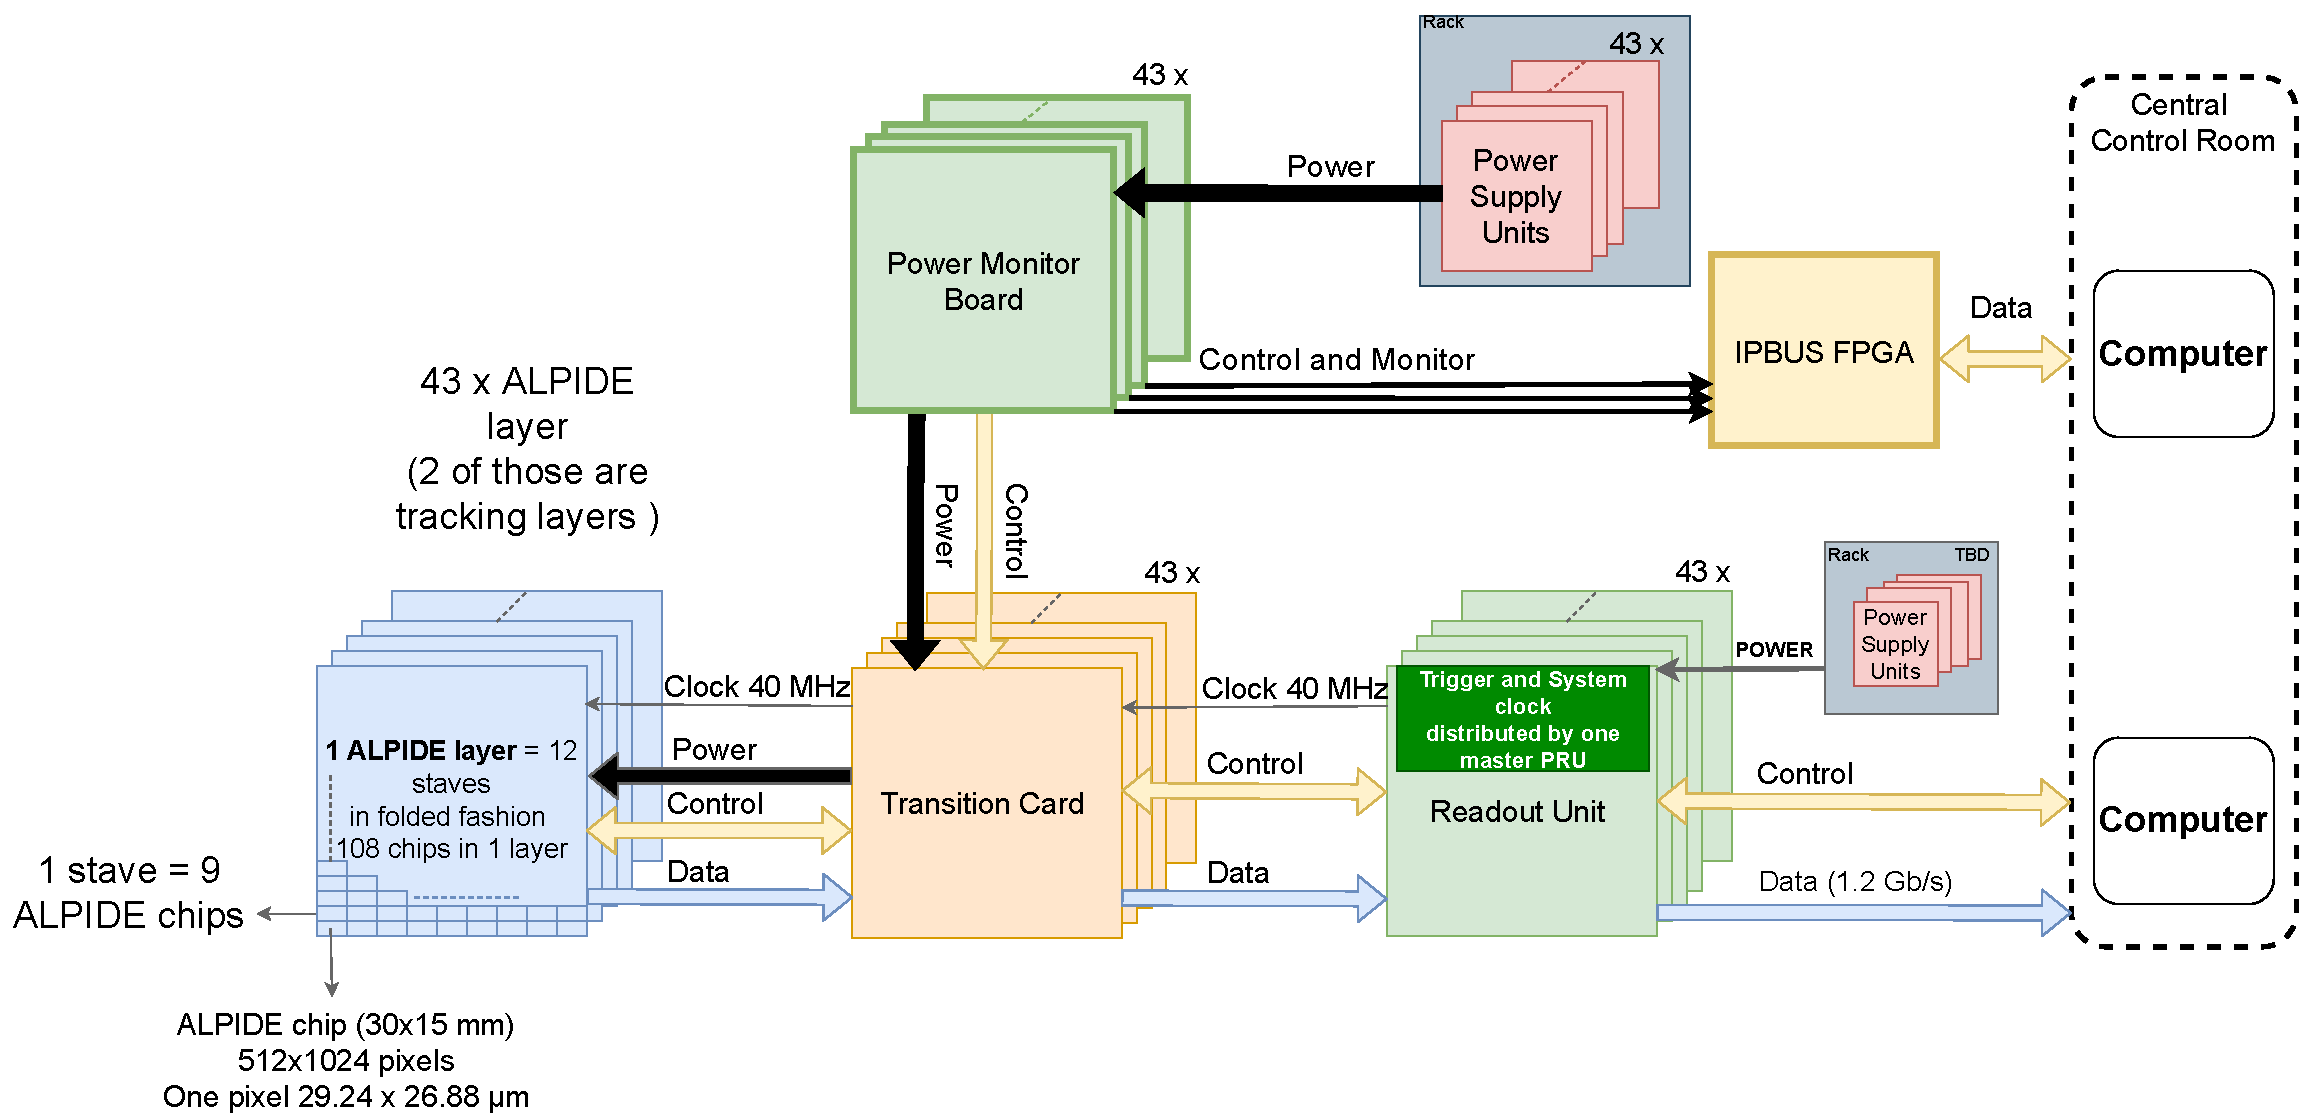
\includegraphics[scale=0.4]{images/pCT_Current_layout-CurrentSystemOverview.pdf}
    \caption{Block diagram of the current design of the pCT system, without the cooling attached. The upper part shows the power delivery and monitoring system, and lower half is the readout unit.}
    \label{fig: pct_diagram}
\end{figure}
\FloatBarrier


\subsection{Digital Tracking Calorimeter}

The \gls{dtc} is the main instrument of the \gls{pct}-system; it combines proton tracking and energy measurement into one technology. It is made out of 43 layers of pixel detectors, where two layers in the rear are used to track the trajectory of the protons and the other 41 measures their energy. A model of it is given in \autoref{fig: dtc_intro}.

A \gls{dtc} is usually realized with front and rear trackers, but only front trackers are used in this prototype. Studies have shown that single-sided proton imaging using Pencil Beam Scanning can lead to similar spatial resolution in the image as compared to double-sided imaging\cite{pbs_result}. The single-sided tracker also comes with a few advantages, such as a lower material budget and less complexity in the rigging of the \gls{dtc}.

The layers of \gls{dtc} are functionally identical. However, the calorimeter layers are made with aluminium absorbers to fully contain the energy range from the proton beam, estimated to be 230 MeV. The tracking layer must have as small a material budget as possible to minimize the scattering of the protons, which can affect the accuracy of the scan. The tracking layers are used to track the angle of the protons that exit the patient; the two layers provide the linear path of the proton, which is used to derive the angle. Based on the angle, one can statistically estimate the most likely path the protons took as they moved through the patient. This statistic is crucial for reconstructing the CT image.

A layer of the \gls{dtc} is realized using 12 strings of \gls{alpide}-chips. A layer comprises two half layers, and a half layer comprises two "slabs" of \gls{alpide}-chips. The "slabs" are three strings glued together; a picture of a half layer is shown in \autoref{fig: half_layer}.

\begin{figure}[!ht]
    \centering
    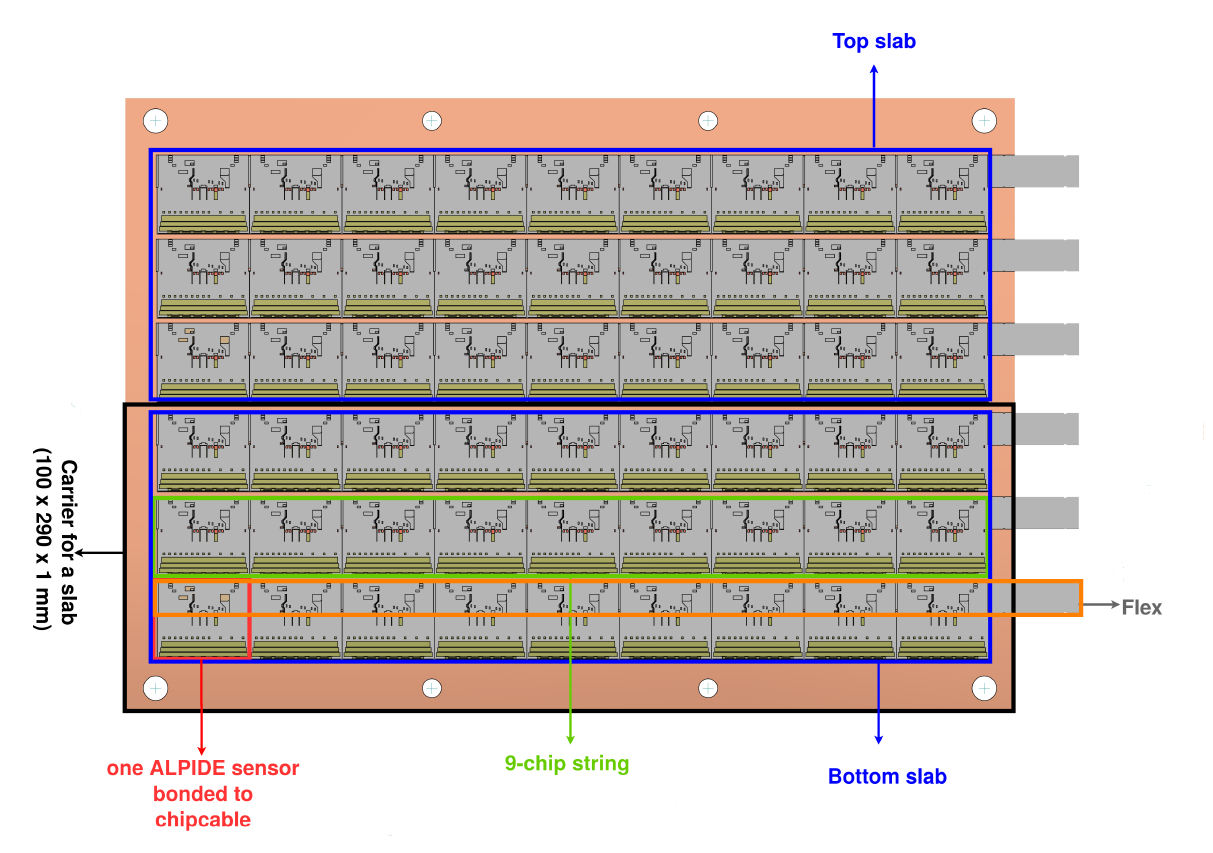
\includegraphics[scale = 0.4]{images/half_tea.png}
    \caption{Image of half sensor layer, highlighting various components.\cite{Tea}}
    \label{fig: half_layer}
\end{figure}


We can note from the half-layer design that the \gls{alpide}-chips only covers about half of the layer; the rest of the space is dedicated to the flex cable. Therefore, two half-layers are stacked so that the \gls{alpide}-chips of one half-layer cover the flex cable of the other, ensuring full area coverage. This gives us a full layer of the \gls{dtc}.


\subsection{ALPIDE chips}

The basic pixel detector sensor used for this project is the \gls{alpide}-chips that were designed for the upgrade of the \gls{its} during the long shutdown of the \gls{lhc} during the 2019-2020 period. The chips are categorized as \gls{maps} with a span of 1.5 cm x 3 cm. The sensor is made of a matrix of 512 x 1024 pixels, which function as binary hit/no hit sensors. A detection threshold is set for the chip, suppressing all hits below the threshold level and functioning as a filter for non-relevant data, such as noise and radiation. A cross-section of the \gls{alpide} silicon is shown in \autoref{fig: alpide_cross}.

\begin{figure}[!htpb]
    \centering
    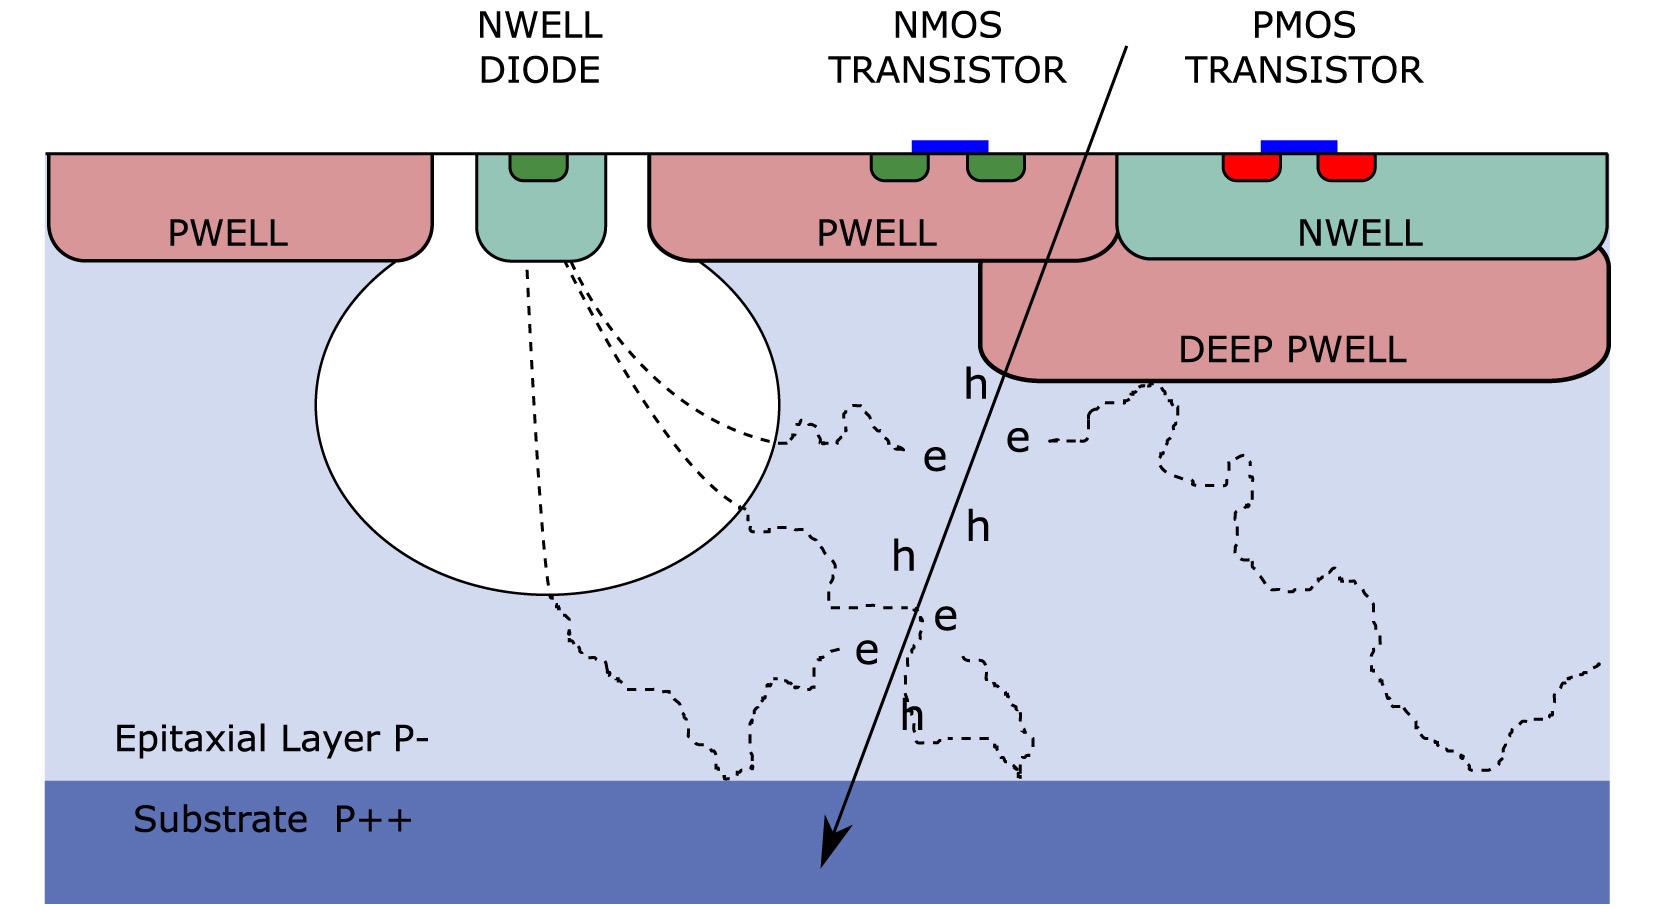
\includegraphics[width=12cm]{images/alpide_chip.jpg}
    \caption{Cross section of an ALPIDE-chip, showing a particle entering the silicon and causing a hit to register.}
    \label{fig: alpide_cross}
\end{figure}
\FloatBarrier


The figure shows a particle entering the silicon and releasing electron-hole pairs from the epitaxial layer. The charge moves through the depletion region and if it reaches the set voltage threshold, a hit is registered in the pixel.

In the \gls{pct} project, nine \gls{alpide}-chips are bonded together on one flex cable, which is defined as one "string". An \gls{alpide} string is shown in \autoref{fig: alpide_physical}.

\begin{figure}[!htpb]
    \centering
    \includegraphics[width=12cm]{images/alpideStringPhysical.png}
    \caption{Image of parts of a string, highlighting the ALPIDE chip, chip cable, and flex cable.}
    \label{fig: alpide_physical}
\end{figure}
\FloatBarrier

The figure shows that half of the string is covered by the chip, and the other half is the flex cable used to mount the chips.

For this thesis, it is also relevant to look at the power consumption of the strings. The \gls{alpide}-chips do not all draw the same amount of current; it is, therefore, necessary to measure the current draw of the strings. A test was performed on a string at the University of Bergen, and it was recorded to draw 880 mA of digital current, and a maximum analog current of 200 mA is also expected. With these measurements, each string requires 1.9V and 1.1A to operate. 


\subsection{Cooling System}

The cooling system consists of two parts, one for the front tracking layers and one for the calorimeter layers. The front tracking layers are liquid-cooled, while the calorimeter layers are cooled using five fans. Figure \ref{fig: cooling_lab} shows lab setup of the cooling system.

\begin{figure}[!ht]
    \centering
    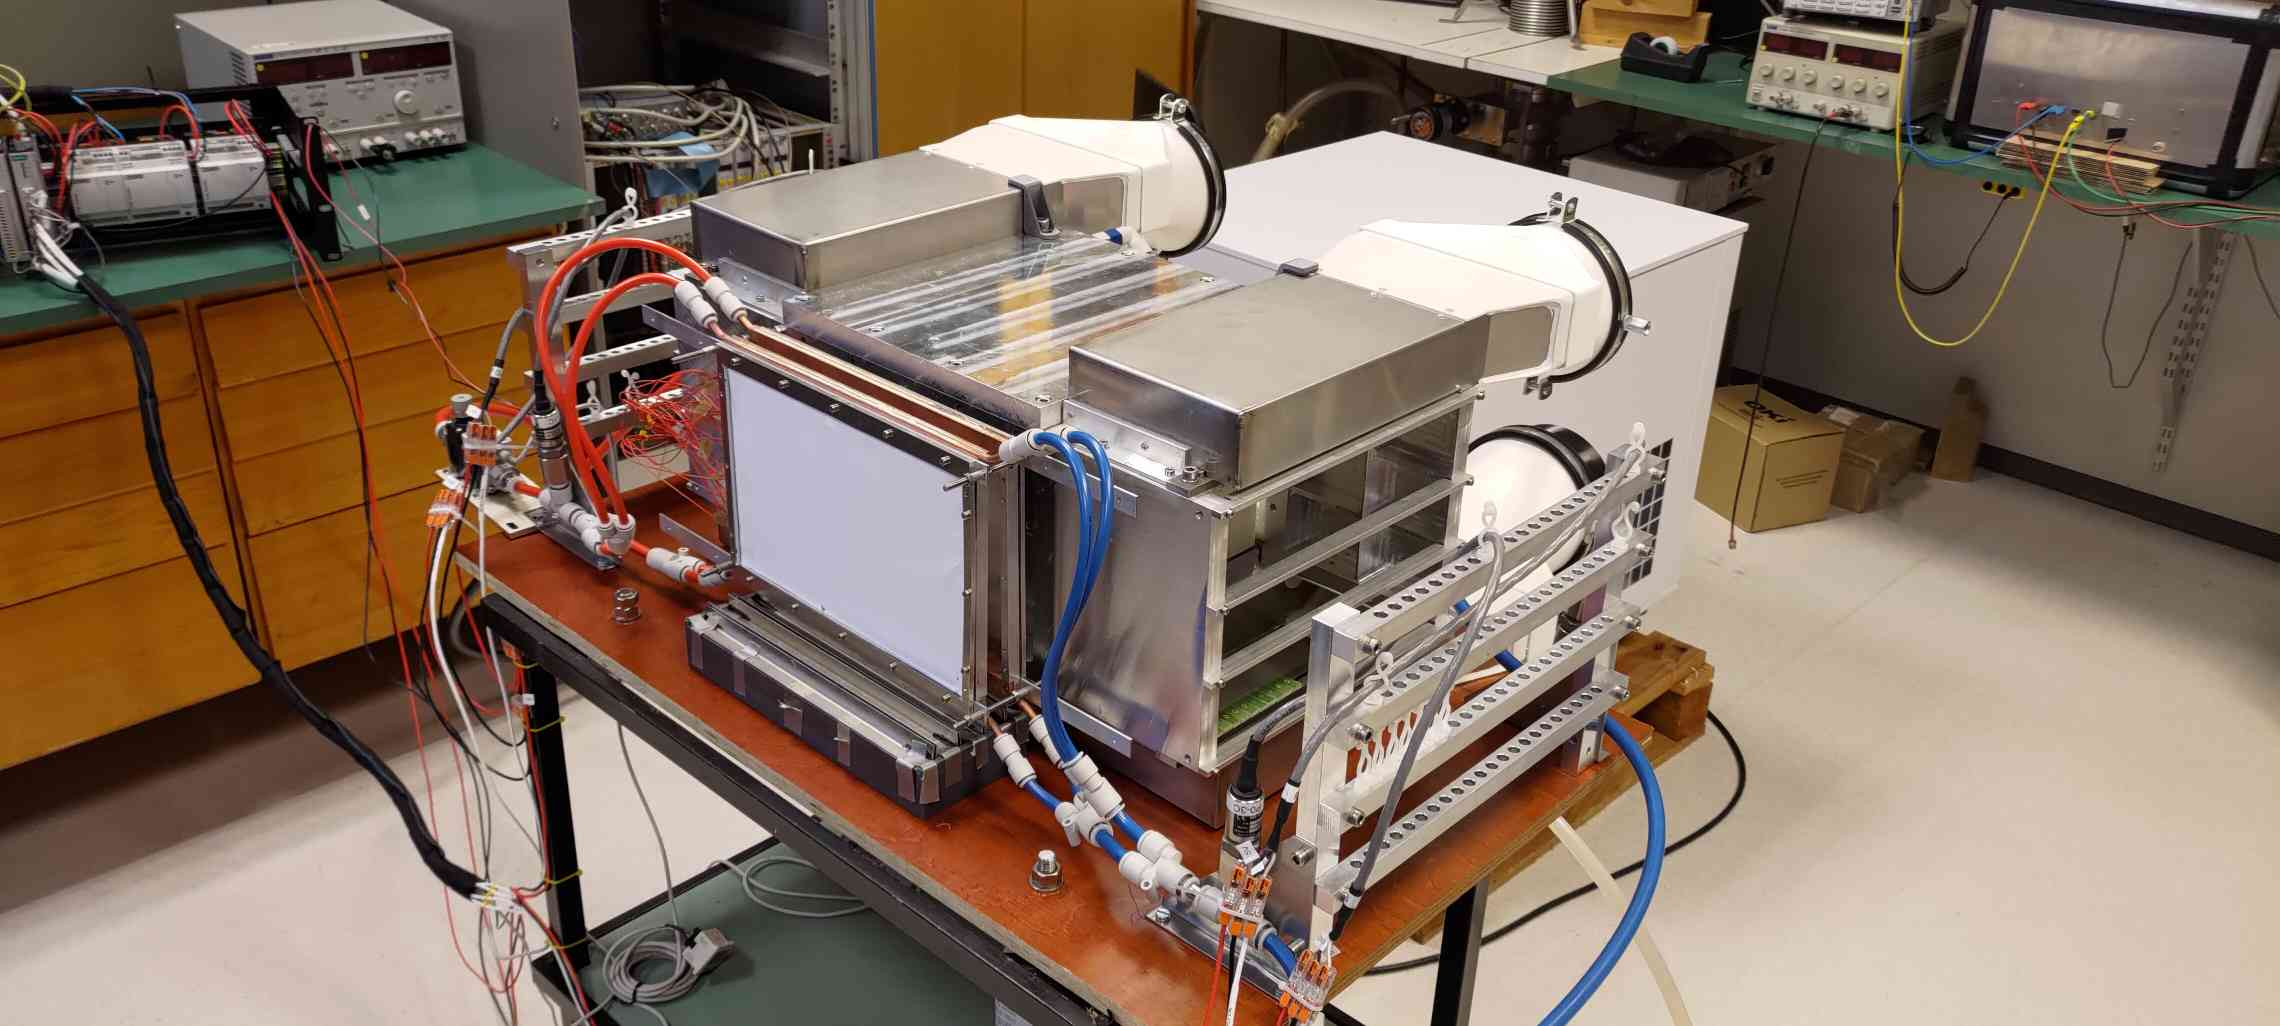
\includegraphics[width=15cm]{images/cooling.jpg}
    \caption{Image of the cooling system in the lab. The front trackers are liquid-cooled and are connected to two flow meters. The fans behind the box serve as the cooling for the calorimeter layers.}
    \label{fig: cooling_lab}
\end{figure}
\FloatBarrier

The cooling control is done through moxa cards, which are connected to the Control Room. The cooling system is monitored with four temperature sensors and two flow meters, and it can also monitor the RPM of the five fans. The control system for the cooling system is still under development; currently, it can only read out values from the sensors.


\subsection{Readout System}

The \gls{pct} readout system comprises 43 readout units, which act as the communication hub between the Control Room and the sensors. Each layer has a corresponding \gls{pru}, which controls the sensors as well as manages the data streams. The \gls{pru} board is realized using an Kintex Ultrascale KU085 \gls{fpga}, and the board is connected to the \gls{tc} using 12 Samtec FireFly cables. A block diagram of the board is shown in \autoref{fig: pru_diagram}.

\begin{figure}[!ht]
    \centering
    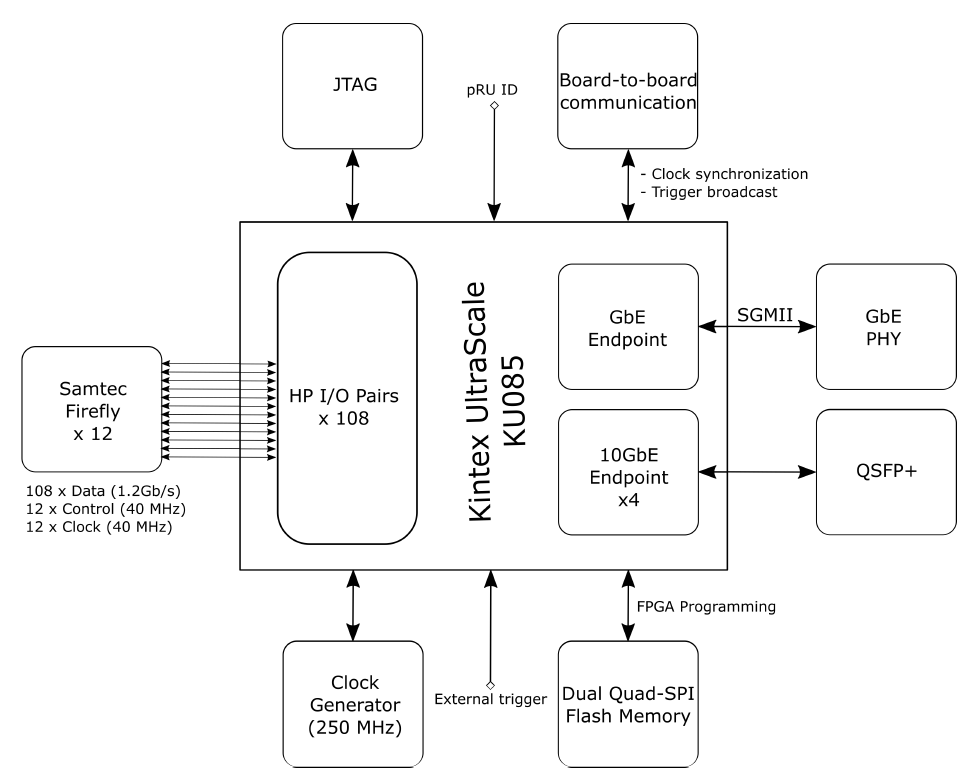
\includegraphics[scale=0.5]{images/pru_diagram.png}
    \caption{Simplified block diagram of the pRU board\cite{ola}}
    \label{fig: pru_diagram}
\end{figure}
\FloatBarrier

There is no monitoring system for the \gls{pru}, but a configuration system exists, which can store configuration values in a database and configure the strings. However, this system requires a new revision to be able to integrate it into the full control system.

\subsection{Power Delivery System}

The power delivery system is responsible for powering the strings on the \gls{dtc} and monitoring the strings' performance. \autoref{fig: pds_diagram} outlines a detailed block diagram of the system.

\begin{figure}[!ht]
    \centering
    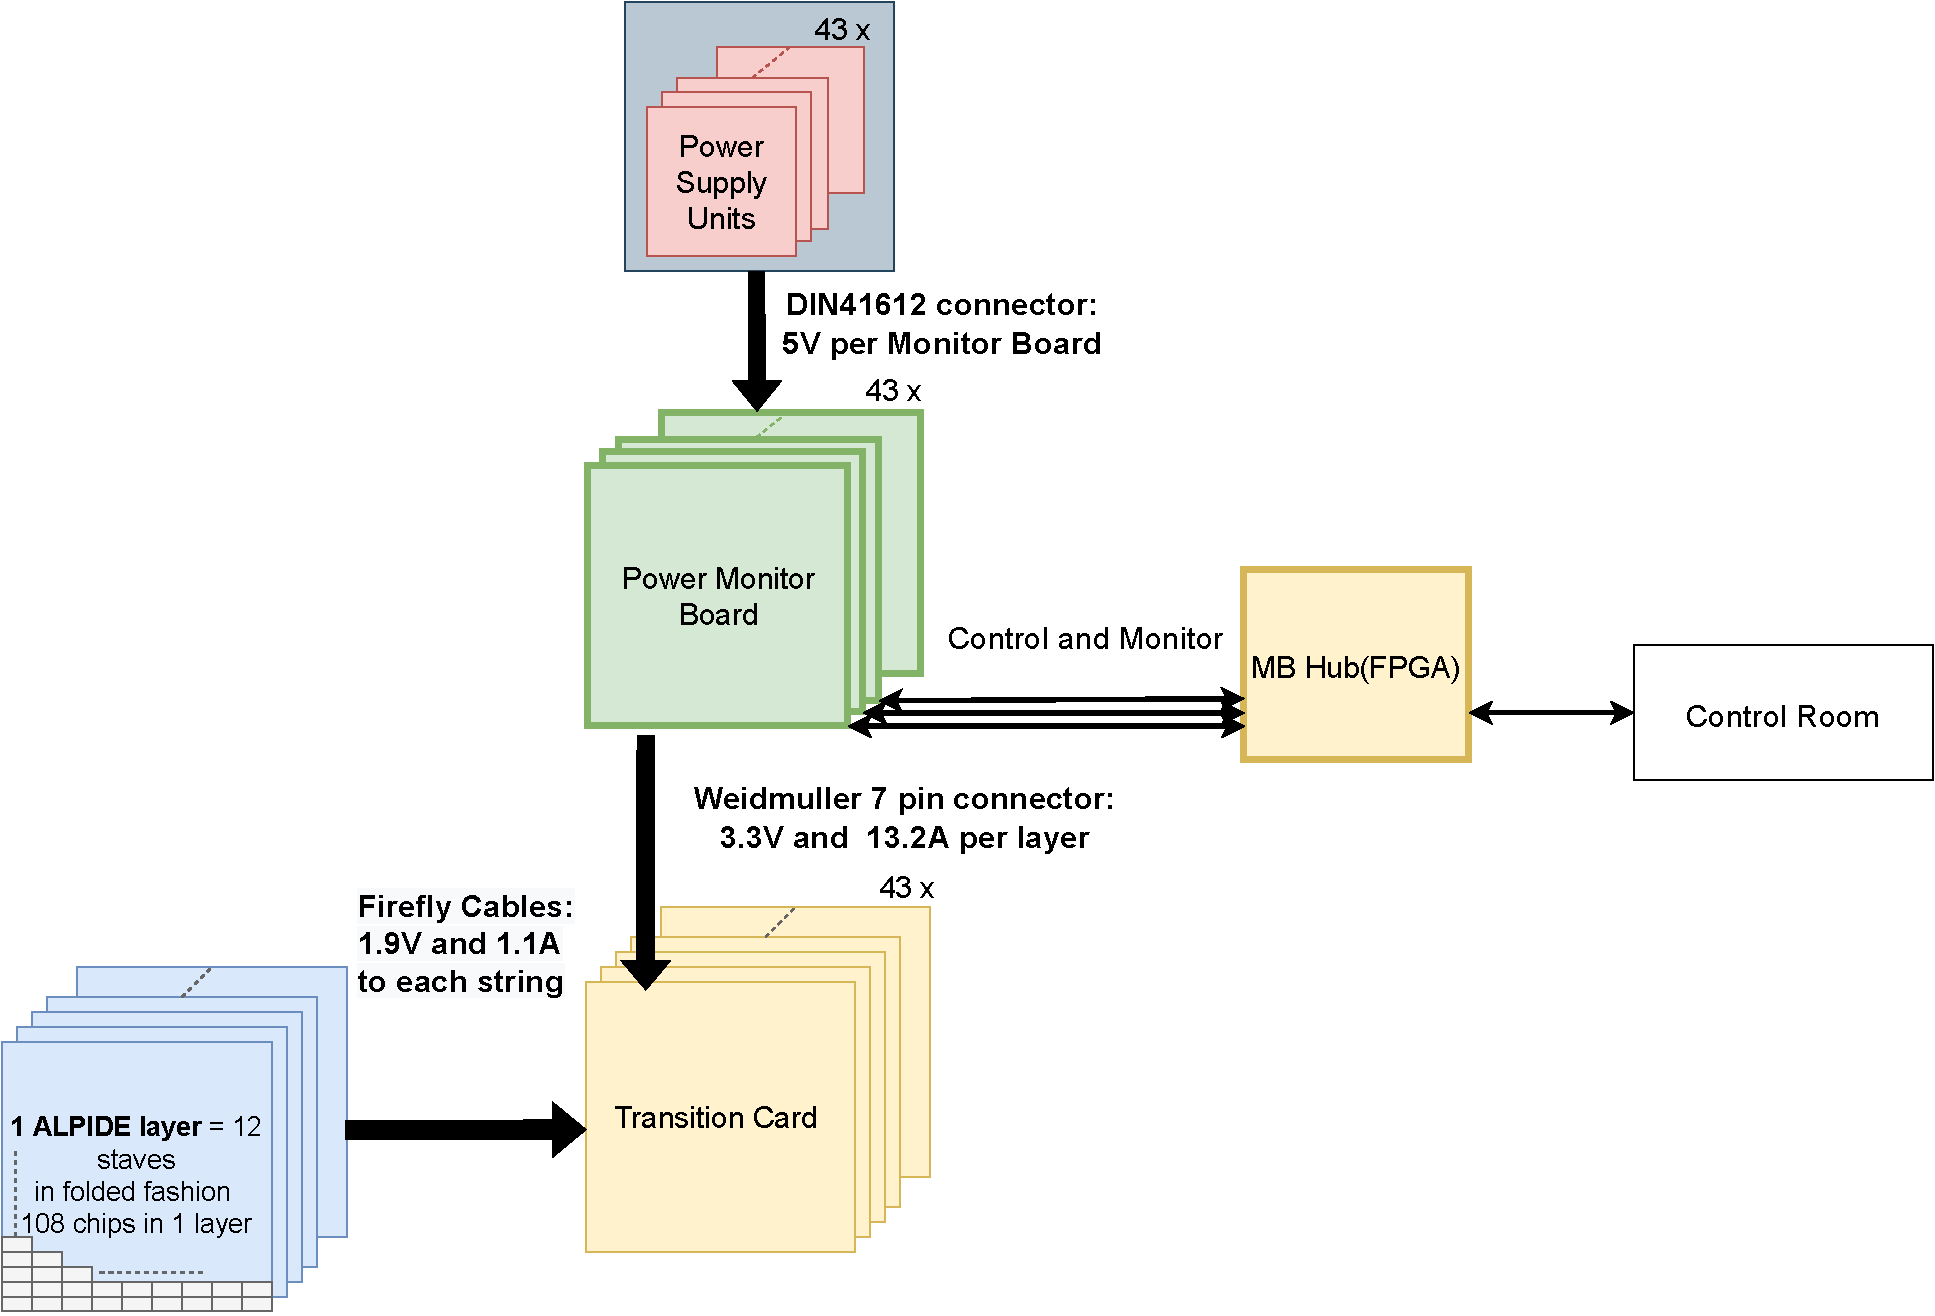
\includegraphics[scale=0.5]{images/pds_detail.pdf}
    \caption{Detailed block diagram of the power delivery system.}
    \label{fig: pds_diagram}
\end{figure}
\FloatBarrier

Control of the system is done through the Control Room, which uses the MB Hub to interface with the \gls{mb}s. The \gls{mb} delivers power from the PSU to the \gls{tc}. It also monitors the temperature and current usage of the strings. A string is turned off by the \gls{mb} if it exceeds the current/temperature threshold. This ensures that the strings are turned off quickly so as to not damage the chips. The \gls{mb}s deliver 3.3V to each \gls{tc}, which uses linear voltage regulators to shift the level down to 1.9V before delivering it to the strings.

The control system of the power delivery is discussed in \autoref{section: pcs}, where the focus is on the communication chain between the Control Room and the \gls{mb}s.



\end{document}